\chapter{MC-SBD-STM Result}

In this chapter, we present the result from the \ac{MC-SBD} algorithm(the algorithm from now) on both the synthetic data and real experimental data on various materials. We first introduce a synthetic QPI-STM data generation process, build a corresponding metric system, and evaluate the performance of the algorithm on a wide range of synthetic data. Then we will show results in the real data, and evaluate it with a simple faithfulness metric. 

\section{MT-SBD-STM Result on synthetic data}
Evaluating the algorithm's performance on synthetic data is necessary, as in the real data we have less access to the ground truth of both kernel and activation. A good synthetic data set should thus capture the physical data generation process during an experiment. In this section, we showcase that the algorithm works well in a wide parameter spaces. We aim to achieve it by presenting an experiment-informed simulation method, build a metric system that evaluates the algorithm from 3 perspectives, and then present results that falls in different parameter spaces. Finally, we will discuss the cases where the algorithm failed and its potential reasons. 

\subsection{Synthetic Data Generation Process}
The synthetic data generation process follow closely with the convolutional model of QPI-STM that we established in Ch. 5. Mathematically, the synthetic data $Y(\omega)$ is generated via:
\begin{equation}
	Y(\omega) = \sum_i^s ( A_i(\omega) * X_i) + \beta. 
\end{equation} 

%A real STM grid map samples from a continuously varying Local density of states. However, due to the discrete nature of computer simulation, we need to make modifications and even compromises in designing the data generation process. 
\begin{figure}
	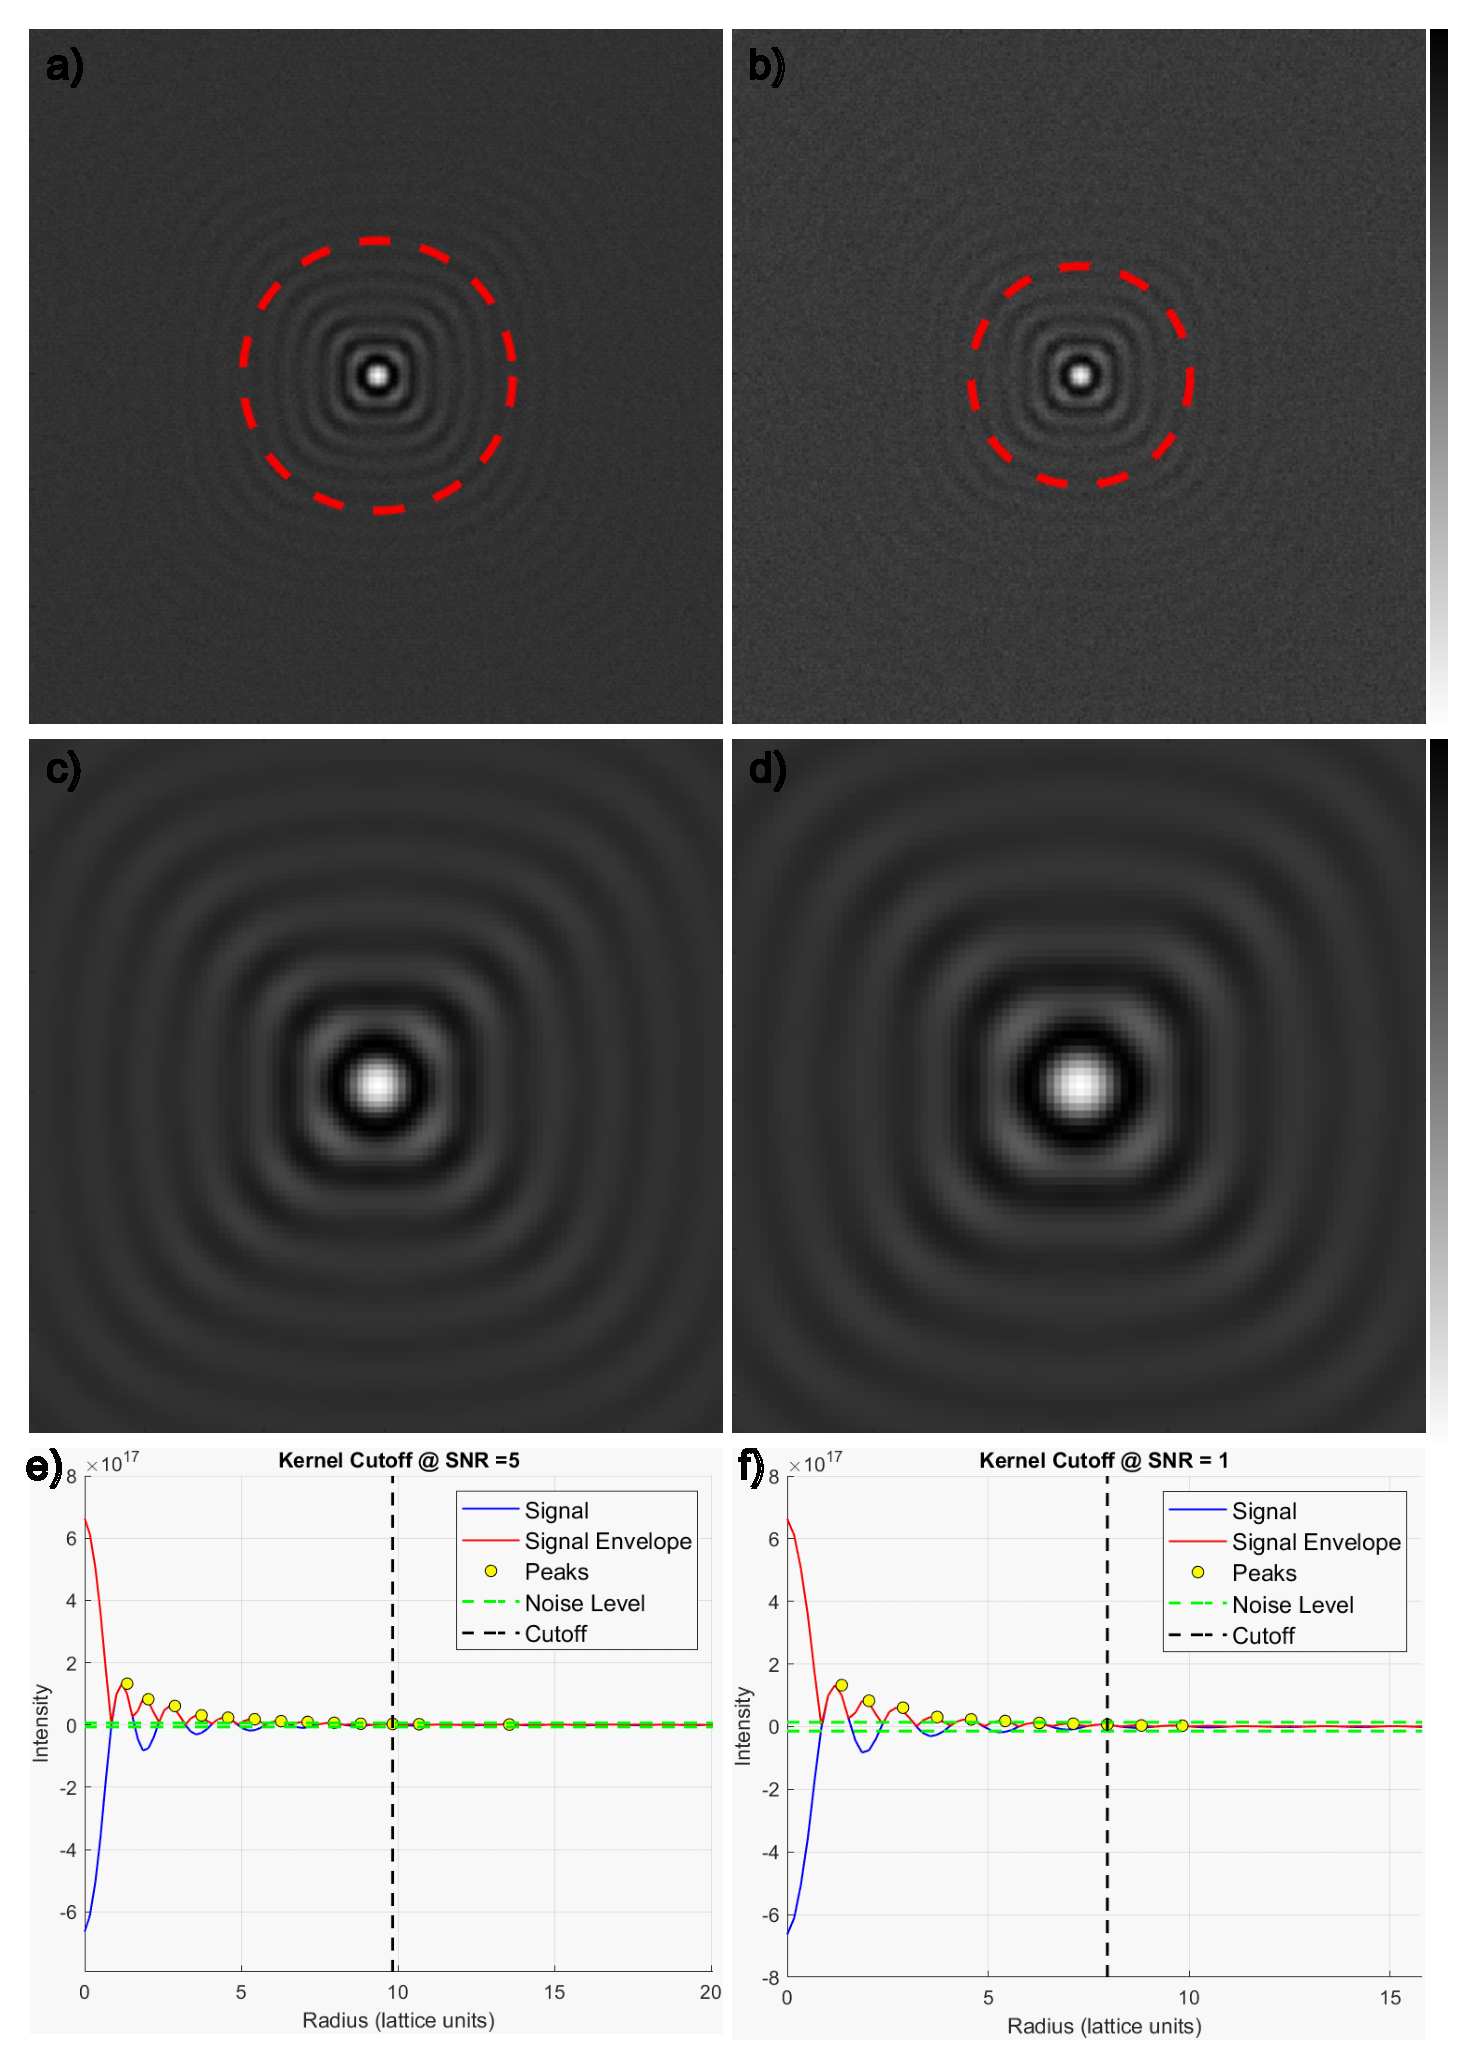
\includegraphics[width= \textwidth]{Ch7_kernel_size.pdf} 
	\centering
	\caption{}
	\label{fig:ch7_kernel_size}
\end{figure}

In practice, there are 4 parameters that dictates $Y(\omega)$, they are:
\begin{itemize}
	\item Signal to Noise Ratio($SNR$): the variance ratio between the noiseless kernel and the noise. This influence $\beta$ and $A_i(\omega)$, we will elaborate the latter influence later. 
	\item Observation lattice size($N_{obs}$): total number of lattice sites per side within the grid map. This dictates the physical size of the grid map. 
	\item Linear observation resolution($p$): number of pixels per lattice site, this is enforced to be an integer due to the discrete nature of simulation. 
	\item defect density($\rho_i$): number of defect i per lattice site. Practically, it is equivalent to the probability of a lattice site to host defect i, a formulation according to the statistical framework of defect we established in Ch. 4.
\end{itemize}
\begin{figure}
	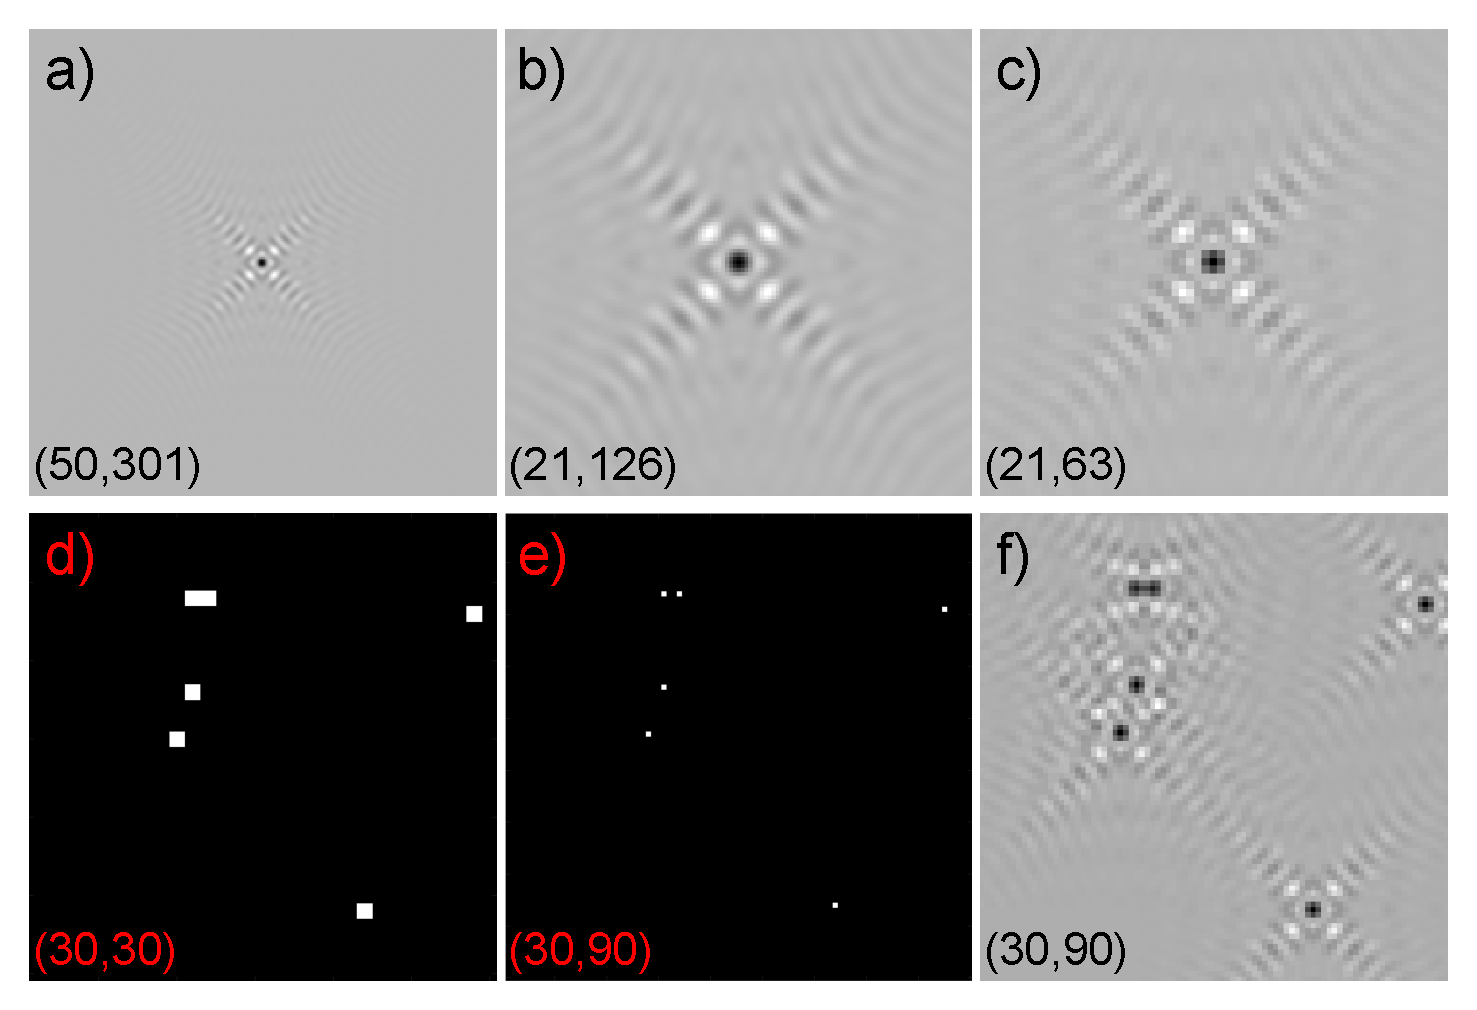
\includegraphics[width= \textwidth]{Ch7_synGen.pdf} 
	\centering
	\caption{}
	\label{fig:ch7syn}
\end{figure}

The step by step data generation process is illustrated in Fig. \ref{fig:ch7syn}. It is worth noting that we have a pair of numbers in the bottom-left corner of each subplot. Every pair indicates the observation lattice size and pixel size of this image. We first take the simulated \ac{LDOS} on the tight-binding model we built in Ch.4 and pick an energy slice, we generate a) with large $N_{obs}$ and dense pixels. Then we choose an an SNR-ratio $SNR$ and apply it onto a), due to the decaying nature of the \ac{QPI} pattern, we can draw an cutoff location where the signals are buried in the noise, as illustrated in Fig. \ref{fig:ch7_kernel_size}. This process gives us b), a truncated version of a) with noise added. a) and b) mimics the underlying \ac{LDOS} on the surface of the sample that \ac{STM} samples from. In real experiment, this sampling process turns the initially continuous \ac{LDOS} to a discrete grid map. Here, we model this processing through down sampling an initially dense grid($p=6$) b) with a smaller linear observation resolution $p=3$ and get c), our ground truth kernel $A^{gt}_i$; note that the down sampling only changes the pixel size, but keeps the spatial lattice size unchanged. The activation map is first generated in the lattice grid, as the impurities mostly sit on the lattice sites. Then we resize the activation map to match the linear resolution of the kernel and get e), our ground truth activation map $X^{gt}_i$. Finally, we use apply 2D linear convolution to $A^{gt}$ and $X^{gt}$ to get the ground truth observation for kernel $i$: $Y^{gt}_i$. We then repeat this process and composite different observations to construct the final observation $Y^{gt}= \sum_iY^{gt}_i$. 

Our simulation approach improves on two key limitations of the original method. First, in the original synthetic data generation workflow proposed by Cheung et al., the kernel was generated by simply selecting a target size and applying imresize to a large single-defect QPI simulation. This process arbitrarily rescales the entire QPI pattern without considering how far the signal meaningfully extends, leading to unphysical distortion of spatial features. In contrast, our method determines the kernel size based on where the QPI signal becomes indistinguishable from noise, with a defined SNR threshold. This ensures the kernel reflects the true spatial extent of the physically meaningful signal. Second, Cheung et al. placed impurities on a binary pixel grid without regard to the underlying lattice, allowing the impurities to appear off-site—a simplification that breaks down in most materials where defects are confined to lattice points. Our method instead defines the activation map on the actual lattice grid and ensures defects are positioned only at valid lattice sites. These two improvements—grounding the kernel in real signal decay and enforcing lattice-consistent activation—make our simulated data more faithful to experimental conditions and more reliable for algorithm benchmarking.

We now show some examples of the synthetic data generated to give some taste to the readers about how we tune the knobs and model datasets in different regimes. As illustrated in Fig. \ref{fig:synexample}, we first plot a reference observation $Y_a$ in a), with 2 different types of defects, $SNR = 5$, $N_{obs}=50$, linear resolution $p = 3$, density of individual type $\rho_i = 0.2 \%$. We can tune the density of individual defect type by changing $\rho_i$, an example is given in b), with $\rho_i$ doubled and other parameters unchanged. We can also tune the spatial resolution of the scan, by changing the linear resolution $p$, in c), we present a case where $p$ is doubled, modeling a case where we have grid map that is more fine-grained. Lastly, we can change the expand the physical coverage of the scan by modifying $N_{obs}$. Here, we doubled the $N_{obs}$ and plot the $Y_d$ in d). With these parameters, we can create a parameter space that covers a wide range of different datasets and then test the robustness of our algorithm. Before we do that, we first need to build a metric system that measures the goodness of reconstruction between the algorithm output and the ground truth data. 

\begin{figure}
	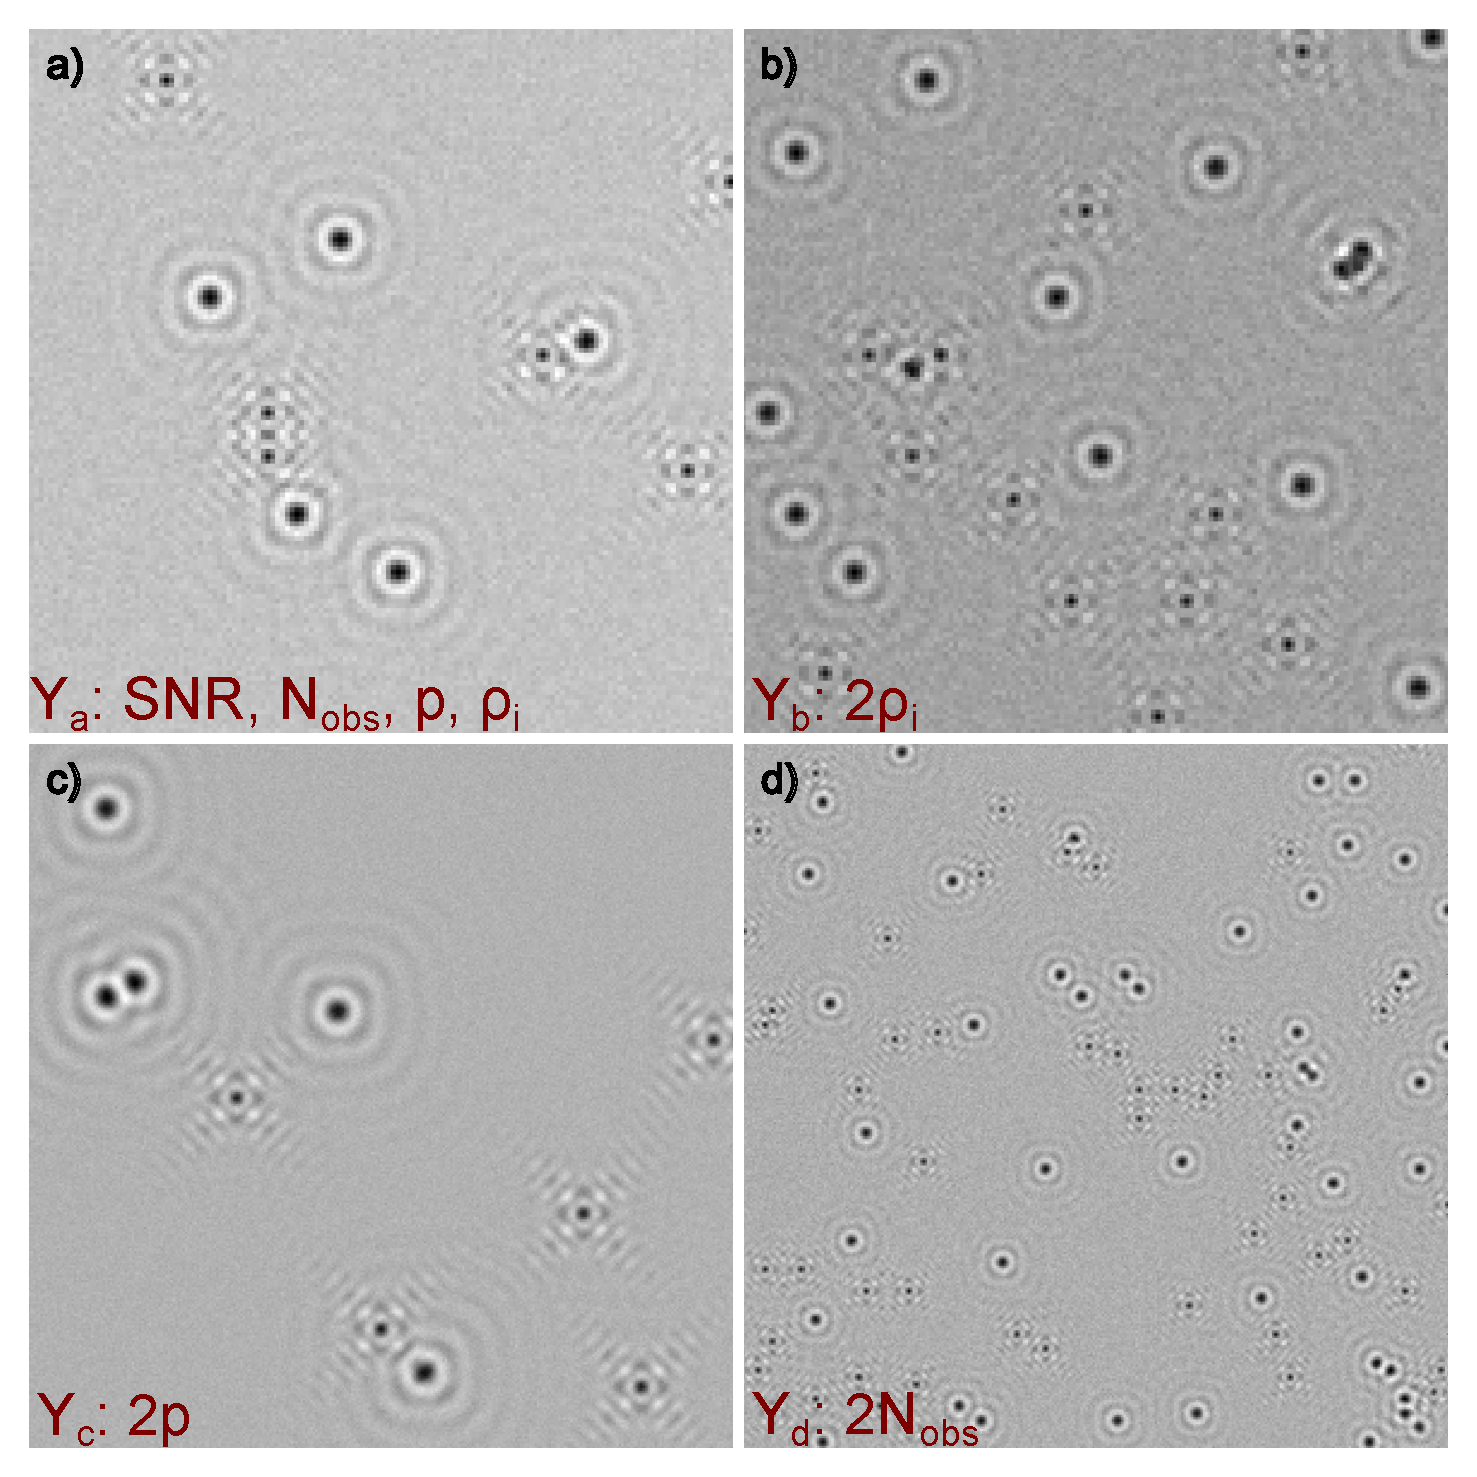
\includegraphics[width= \textwidth]{synGenExamples.pdf} 
	\centering
	\caption{}
	\label{fig:synexample}
\end{figure}

\section{MT-SBD-STM Metric system}
The MT-SBD metric system consists of 4 metrics. They are \textbf{Kernel Similarity(KS)}, \textbf{Activation Similarity(AS)}, \textbf{Demixing score(DS)}, and \textbf{Observation fidelity(OF)}. \textbf{KS} and \textbf{AS} requires the ground truth data, which can only be accessed in synthetic data, the rest of metrics can be applied to both synthetic data and real data. We will illustrate these 4 metrics through an example run of the algorithm on a synthetic observation. 

\subsection{Tune-able parameter space}

\section{Benchmark tests on the parameter space}
\subsection{sparsity}
\subsection{Number of defect types}
\subsection{spatial resolution and noise level}

\section{MC-SBD-STM on real data}
\subsection{real data complexity}
\subsection{preprocessing pipelines}
\subsection{Ag}
\subsection{ZrSiTe}
\subsection{PtSn4}
\subsection{Potential use in other materials}

\section{Conclusion}
\subsection{regime it works and doesn't}
\subsection{Recipe to take data for MC-SBD}
\subsection{Future directions}